\documentclass[11pt]{article}

\usepackage[T1]{fontenc} 
\usepackage[english,spanish]{babel} 	
\usepackage{hyperref}  
\usepackage{url}
\usepackage{mathptmx}
\usepackage{amsmath}
\usepackage{mathtools}
\usepackage{mathrsfs}
\usepackage{amssymb}
\usepackage{cancel} 
\usepackage{graphicx} 
\usepackage{geometry}
\usepackage{csquotes}
\usepackage{courier}
\usepackage[framemethod=TikZ]{mdframed} 
\usepackage{booktabs}
\usepackage{listings}

 \geometry{
 a4paper,
 total={210mm,297mm},
 left=20mm,
 right=20mm,
 top=20mm,
 bottom=20mm,
 }

\mdfdefinestyle{MyFrame}{%
    linecolor=black,
    outerlinewidth=0.3pt,
    roundcorner=7pt,
    innertopmargin=\baselineskip,
    innerbottommargin=\baselineskip,
    innerrightmargin=20pt,
    innerleftmargin=20pt,
    backgroundcolor=gray!12!white}

\graphicspath{{images/}}


\title{New aperture model for the collimation routine BeamLossPattern}
\author{Andrea Santamar\'ia Garc\'ia}

\begin{document}
\usefont{T1}{cmr}{m}{n}
\selectlanguage{english}
\hypersetup{linkbordercolor=blue}
\maketitle
\tableofcontents

\section{BeamLossPattern}
\begin{mdframed}[style=MyFrame]
\hyphenblockcquote{english}{website}{
BeamLossPattern is a program that calculates the location of particle losses along an accelerator. It relies on an aperture model of the full machine and takes as an input the particle coordinate as a function of the longitudinal coordinate (referred to as particle trajectories). 
Locations of beam losses are identified with a spatial resolution of 10 centimetres. For the 27 km long LHC ring, this is equivalent to checking 270000 loss locations! This is achieved by interpolating trajectories between to consecutive lattice elements (typical distance up to > 100 m).
The LHC aperture model has mostly been set by using that MADX interfaces with the LHC layout database. However, several aperture definitions required the preparation of dedicated MADX scripts in order to complement missing information on the database (see below).
It is noted that the program BeamLossPattern is completely independent on MADX. MADX is only used to generate input files for the aperture program (aperture definitions versus longitudinal coordinate, survey files with the position of the design orbit, closed-orbit distortions, etc...). In particular, this means that the generated MADX scripts have not been conceived for MADX users: detailed MADX studies (e.g., particle tracking, APL aperture studies) might require different optimization such as positioning of aperture definition markers, definitions of aperture for specific elements, etc.
For the moment, the aperture model for the LHC optics version V6.5 (sequence) contains:

\begin{enumerate}
\item Beam screen location for all cold elements (form database)
\item Aperture definition for the cold elements within beam screen markers (MADX script)
\item Aperture definitions for warm elements (warm)
\item Aperture of the various BPM types (BPM)
\item Experimental regions (IR1, IR2, IR5, IR8)
\item Standard aperture definition of the vacuum chambers - no flange position (drifts)
\item Fixing by hand some special elements (fix holes)
\end{enumerate}

\textbf{Known missing elements}: Recombination chambers, position of vacuum chamber flanges of IR6 kickers.

\textbf{Remark}: It is noted that the aperture of collimators and protection devices are not included in the aperture model of the ring. The reason for this choice is that the treatment of these elements is carried out within the tracking code, which provides directly the number of impacting particles on the collimators and the locations of inelastic impacts within the volume of the collimator jaws. 
Therefore, the aperture of the above 'injection' and 'lowb' lattices are identical (movable elements with different settings at injection or top energy are the only aperture differences that can arise). Different names for the two cases are kept for compatibility with the BeamLossPattern input.

The BeamLossPattern program does recognize square apertures and hence collimators can easily be modelled if needed. 

Aperture types accepted by the program (RECTELLIPSE notation, see MADX manual): Circle, square, ellipse, LHC beam screen, RaceTrack.
}
\end{mdframed}

\clearpage
 
\section{GetAperture}
\begin{mdframed}[style=MyFrame]
\hyphenblockcquote{english}{website}{For a given lattice and aperture model, this program produces an ascii files with the aperture every 10 cm all along the beam line. Aperture values are given at three different azimuthal angles: 0, pi/4 and pi/2. In order to be able to calculate the aperture in any position along the considered metre (and not only at the positions where the aperture is defined) the member function "GetAperture(double p)" can be used.
It calculates the aperture as interpolation of the point where the aperture has been defined.}
\end{mdframed}

In order to test the GetAperture routine, the file \texttt{allapert\_hllhc\_2013.09.04.b1} was used. This file was originally generated in 2008 and includes the optics version V6.5. We can see from the plots that the GetAperture routine gets rid of the zero values of the aperture. We can also see that in interpolates the aperture at different values than the original one (see IP3 and 7 in the y coordinate).

\begin{minipage}{0.47\linewidth}
\includegraphics[width=\linewidth]{allapert_ip_1_x.png}
\end{minipage}
\begin{minipage}{0.47\linewidth}
\includegraphics[width=\linewidth]{allapert_ip_1_y.png}
\end{minipage}

\begin{minipage}{0.47\linewidth}
\includegraphics[width=\linewidth]{allapert_ip_2_x.png}
\end{minipage}
\begin{minipage}{0.47\linewidth}
\includegraphics[width=\linewidth]{allapert_ip_2_y.png}
\end{minipage}

\begin{minipage}{0.47\linewidth}
\includegraphics[width=\linewidth]{allapert_ip_3_x.png}
\end{minipage}
\begin{minipage}{0.47\linewidth}
\includegraphics[width=\linewidth]{allapert_ip_3_y.png}
\end{minipage}

\begin{minipage}{0.47\linewidth}
\includegraphics[width=\linewidth]{allapert_ip_4_x.png}
\end{minipage}
\begin{minipage}{0.47\linewidth}
\includegraphics[width=\linewidth]{allapert_ip_4_y.png}
\end{minipage}

\begin{minipage}{0.47\linewidth}
\includegraphics[width=\linewidth]{allapert_ip_5_x.png}
\end{minipage}
\begin{minipage}{0.47\linewidth}
\includegraphics[width=\linewidth]{allapert_ip_5_y.png}
\end{minipage}

\begin{minipage}{0.47\linewidth}
\includegraphics[width=\linewidth]{allapert_ip_6_x.png}
\end{minipage}
\begin{minipage}{0.47\linewidth}
\includegraphics[width=\linewidth]{allapert_ip_6_y.png}
\end{minipage}

\begin{minipage}{0.47\linewidth}
\includegraphics[width=\linewidth]{allapert_ip_7_x.png}
\end{minipage}
\begin{minipage}{0.47\linewidth}
\includegraphics[width=\linewidth]{allapert_ip_7_y.png}
\end{minipage}

\begin{minipage}{0.47\linewidth}
\includegraphics[width=\linewidth]{allapert_ip_8_x.png}
\end{minipage}
\begin{minipage}{0.47\linewidth}
\includegraphics[width=\linewidth]{allapert_ip_8_y.png}
\end{minipage}

\section{New aperture model with HLLHCV1.0 optics}
First attempts of generating a new allapert file are described below. The code can be found here \cite{github}.
\subsection{With vacuum markers and experimental beampipe}
\lstinputlisting[breaklines=true, frame=single, basicstyle=\ttfamily\footnotesize, numbers=left, language=C++, commentstyle=\color{blue}\ttfamily,keywordstyle=\color{blue}\ttfamily, stringstyle=\color{purple}\ttfamily, showstringspaces=false]{1.madx}

\vspace{50pt}

The Twiss file generated with this command is not an appropiate input for GetAperture, since it gives segmentation fault when executed. It apparently doesn't support the CIRCLE aperture type as defined in MAD-X \cite{mad_ap} (although the documentation says it does \cite{website}).

\begin{lstlisting}[frame=single, basicstyle=\ttfamily\footnotesize, numbers=left] 
ERROR: Invalid aperture definition!!
0.0235 0 0 0 
ERROR: Invalid aperture definition!!
0.029 0 0 0 

All aperture information has been read and the sequence has been created!

Length of the read sequence: 26659 metres.

Special case: aperture definitions at 0 and 0 are identical!
Segmentation fault
\end{lstlisting}
\vspace{20pt}

Further testing reveals that it doesn't support RACETRACK either:
\begin{lstlisting}[frame=single, basicstyle=\ttfamily\footnotesize, numbers=left] 
./GetAperture allapert_final.b1 
Reading aperture file allapert_final.b1

Reading from "allapert_final.b1"
Total number of read elements: 11446

ERROR: Invalid aperture definition!!
0 0.017 0.033 0 
ERROR: Invalid aperture definition!!
0 0.01375 0.03375 0 
ERROR: Invalid aperture definition!!
0 0.01375 0.03375 0 

All aperture information has been read and the sequence has been created!

Length of the read sequence: 26659 metres.

Special case: aperture definitions at 0 and 0 are identical!
Special case: aperture definitions at 0 and 0 are identical!
Special case: aperture definitions at 0 and 0 are identical!
Special case: aperture definitions at 0 and 0 are identical!
Special case: aperture definitions at 0 and 0 are identical!
Special case: aperture definitions at 0.5 and 0.5 are identical!
Special case: aperture definitions at 0.5 and 0.5 are identical!
Segmentation fault
\end{lstlisting}
\vspace{20pt}

Since it only seems to support aperture with the four parameters defined, I create a Python script that will transform CIRCLE and RACETRACK into RECTELLIPSE:

\lstinputlisting[breaklines=true, frame=single, basicstyle=\ttfamily\footnotesize, numbers=left, language=Python, commentstyle=\color{blue}\ttfamily,keywordstyle=\color{blue}\ttfamily, stringstyle=\color{purple}\ttfamily, showstringspaces=false]{allapert_editor.py}

\vspace{20pt}

This time we get no segmentation fault:
\begin{lstlisting}[frame=single, basicstyle=\ttfamily\footnotesize, numbers=left] 
./GetAperture allapert_final.b1 
Reading aperture file allapert_final.b1

Reading from "allapert_final.b1"
Total number of read elements: 11446


All aperture information has been read and the sequence has been created!

Length of the read sequence: 26659 metres.

Special case: aperture definitions at 0 and 0 are identical!
Special case: aperture definitions at 0 and 0 are identical!
Special case: aperture definitions at 0 and 0 are identical!
Special case: aperture definitions at 0 and 0 are identical!
Special case: aperture definitions at 0 and 0 are identical!
Special case: aperture definitions at 0.5 and 0.5 are identical!
Special case: aperture definitions at 0.5 and 0.5 are identical!
Warning: aperture definition added at the end of the metre!
\end{lstlisting}
\vspace{20pt}

I compare the newly created aperture with the old one, after being processed by GetAperture:

\begin{minipage}{0.47\linewidth}
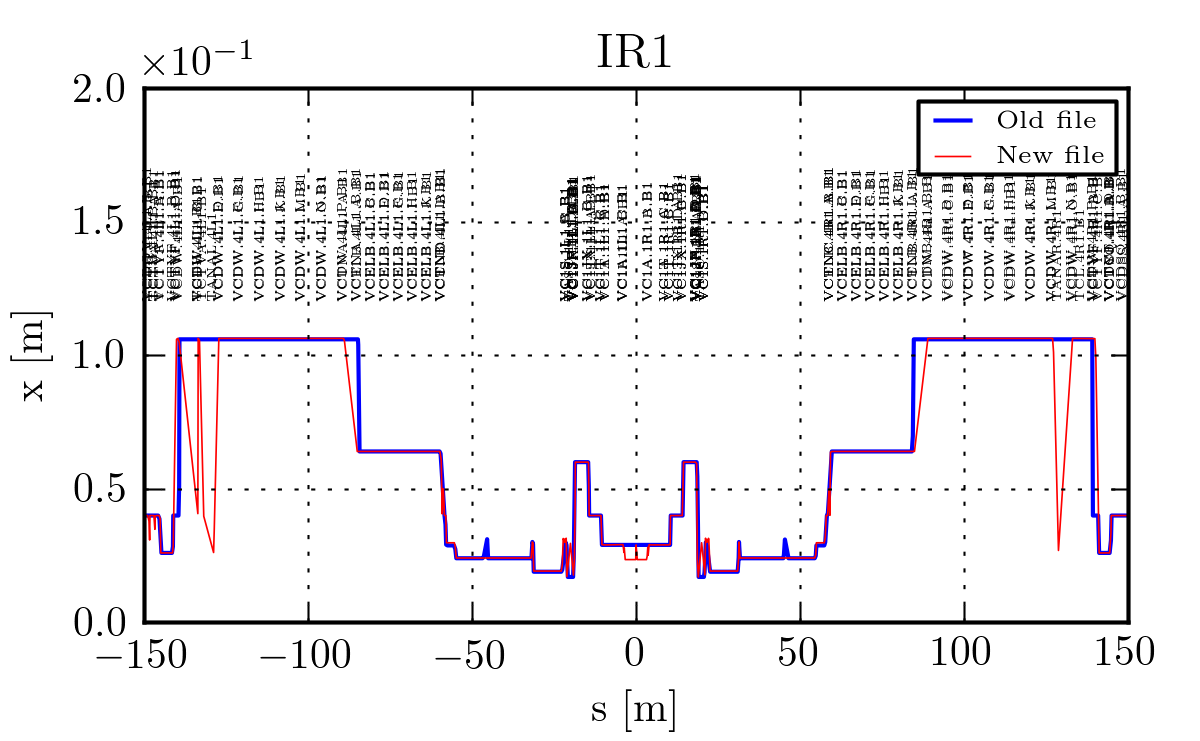
\includegraphics[width=\linewidth]{allapert_ip_1_x_new.png}
\end{minipage}
\begin{minipage}{0.47\linewidth}
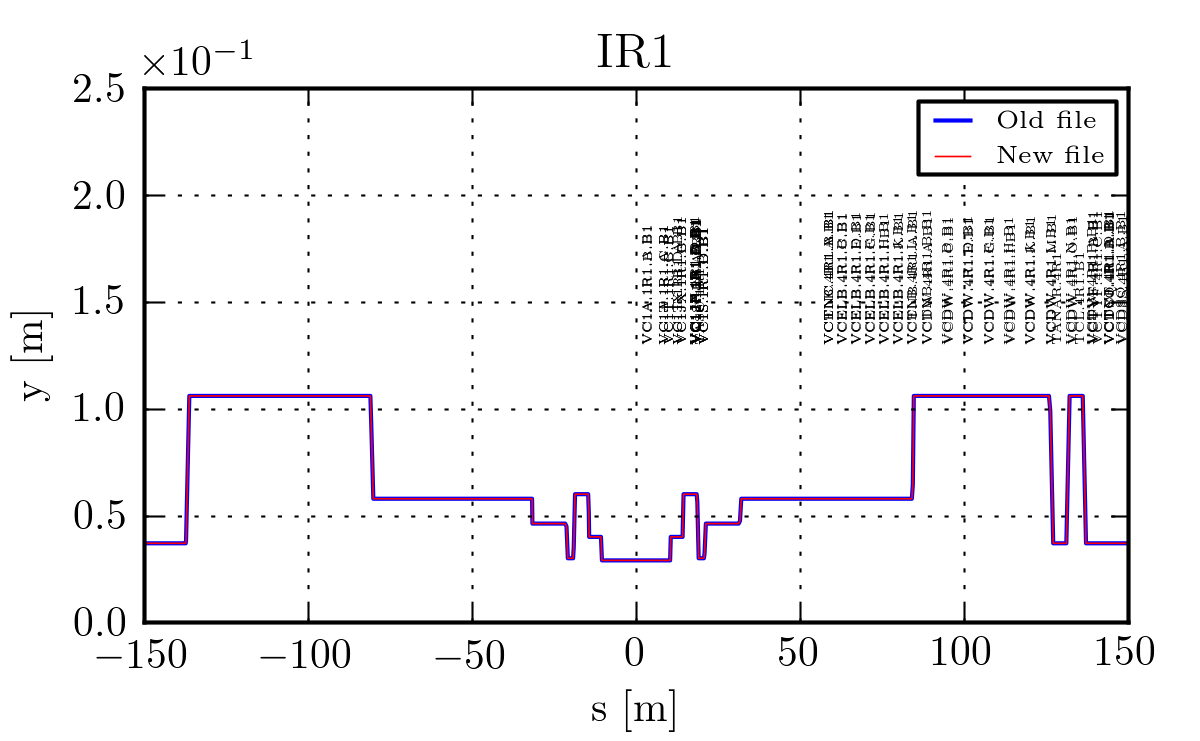
\includegraphics[width=\linewidth]{allapert_ip_1_y_new.png}
\end{minipage}

\begin{minipage}{0.47\linewidth}
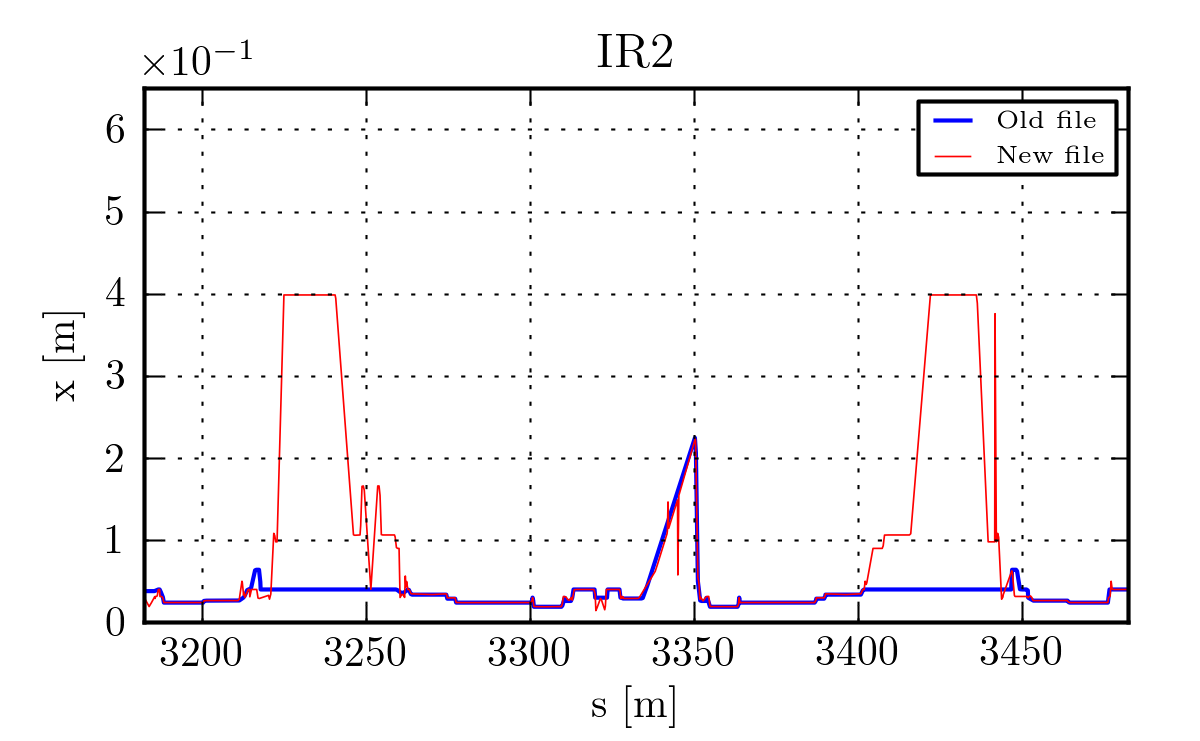
\includegraphics[width=\linewidth]{allapert_ip_2_x_new.png}
\end{minipage}
\begin{minipage}{0.47\linewidth}
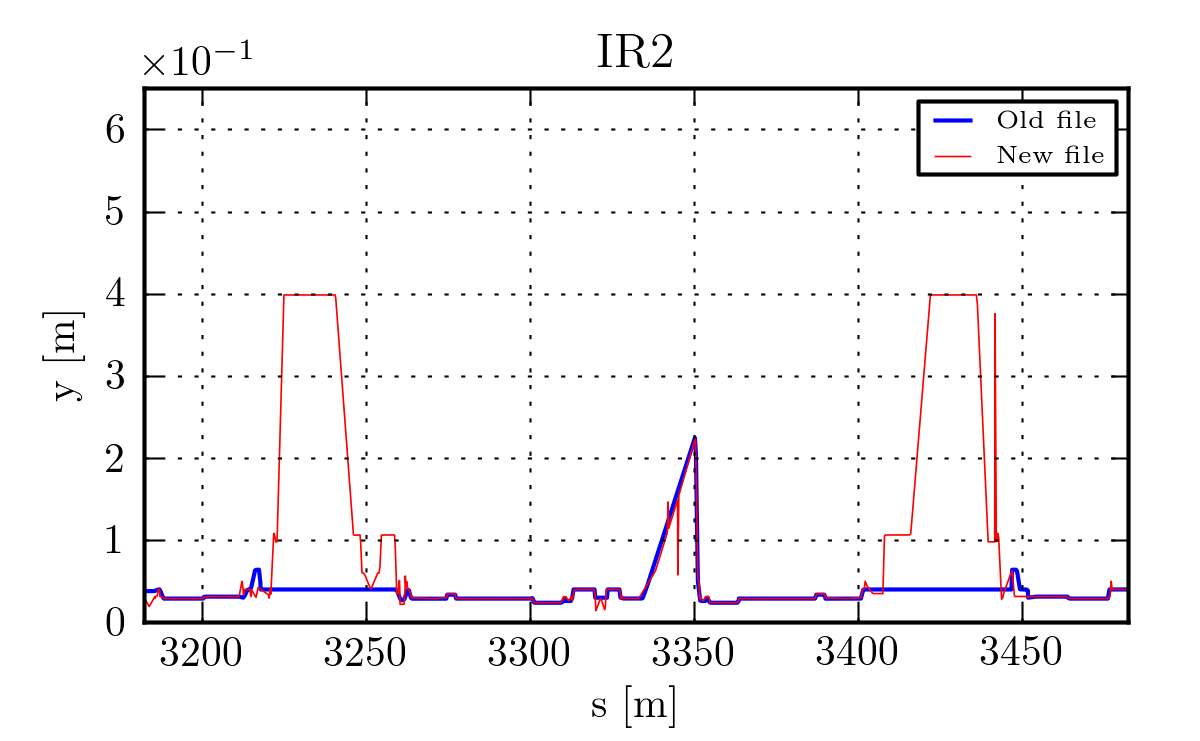
\includegraphics[width=\linewidth]{allapert_ip_2_y_new.png}
\end{minipage}

\begin{minipage}{0.47\linewidth}
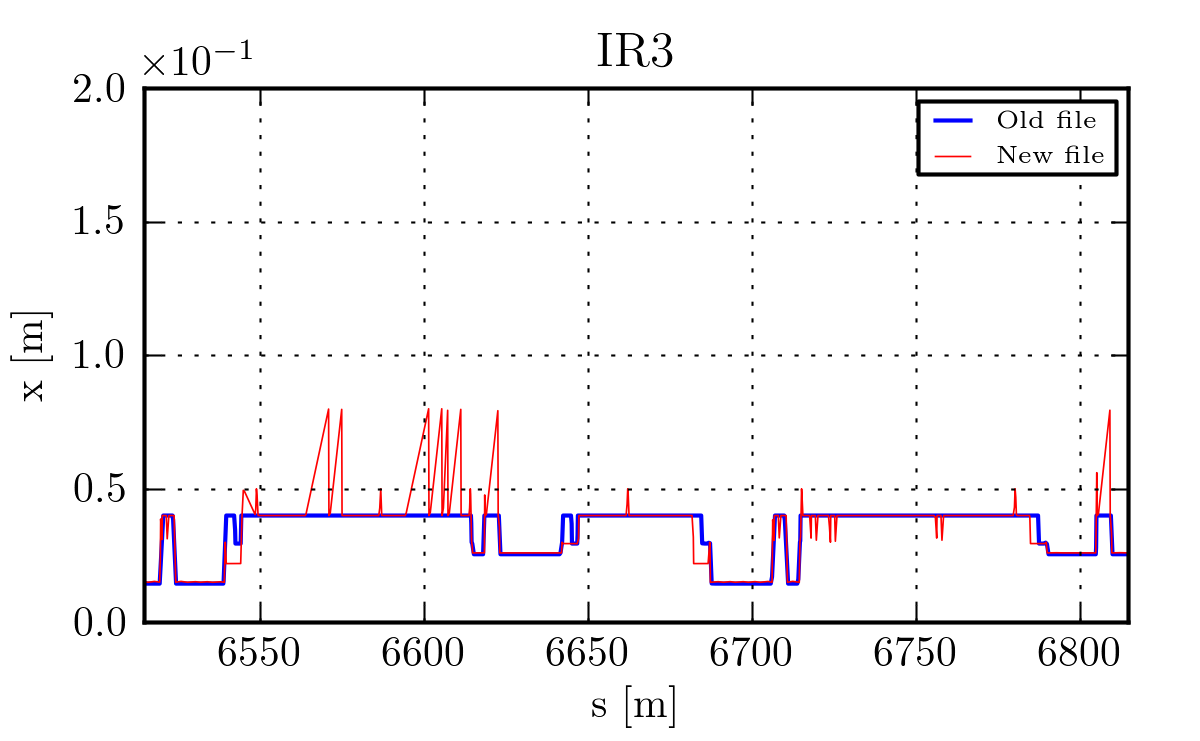
\includegraphics[width=\linewidth]{allapert_ip_3_x_new.png}
\end{minipage}
\begin{minipage}{0.47\linewidth}
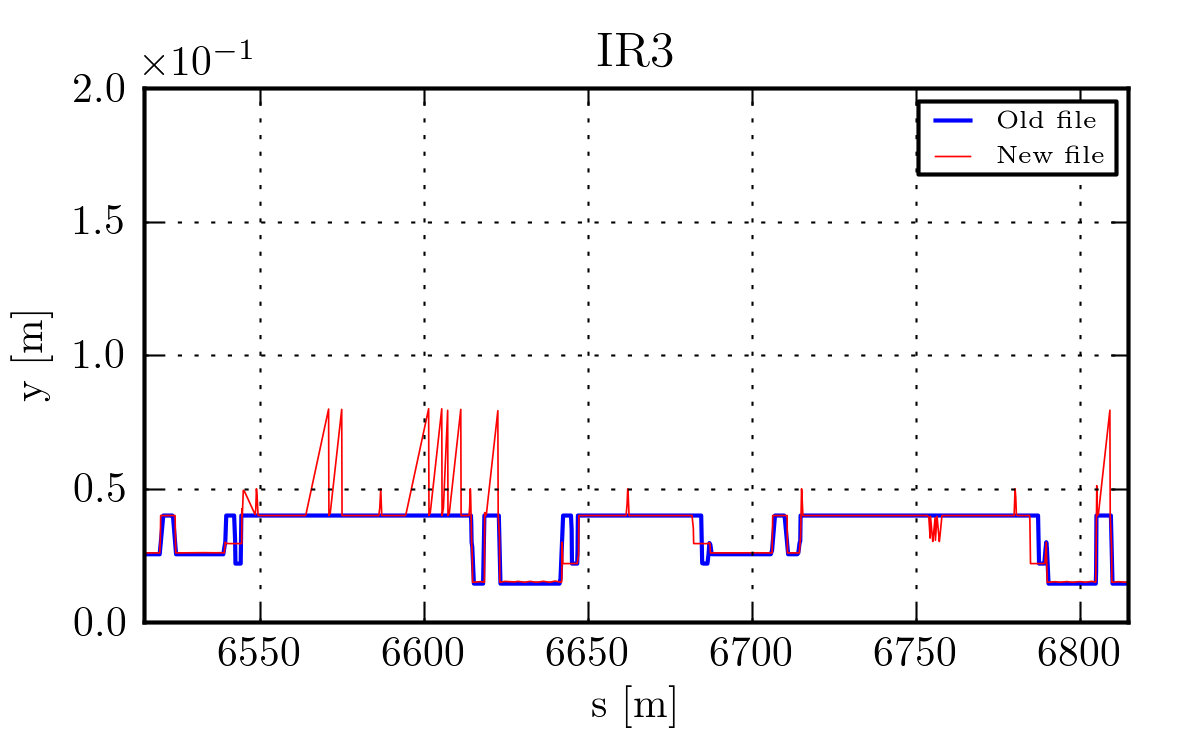
\includegraphics[width=\linewidth]{allapert_ip_3_y_new.png}
\end{minipage}

\begin{minipage}{0.47\linewidth}
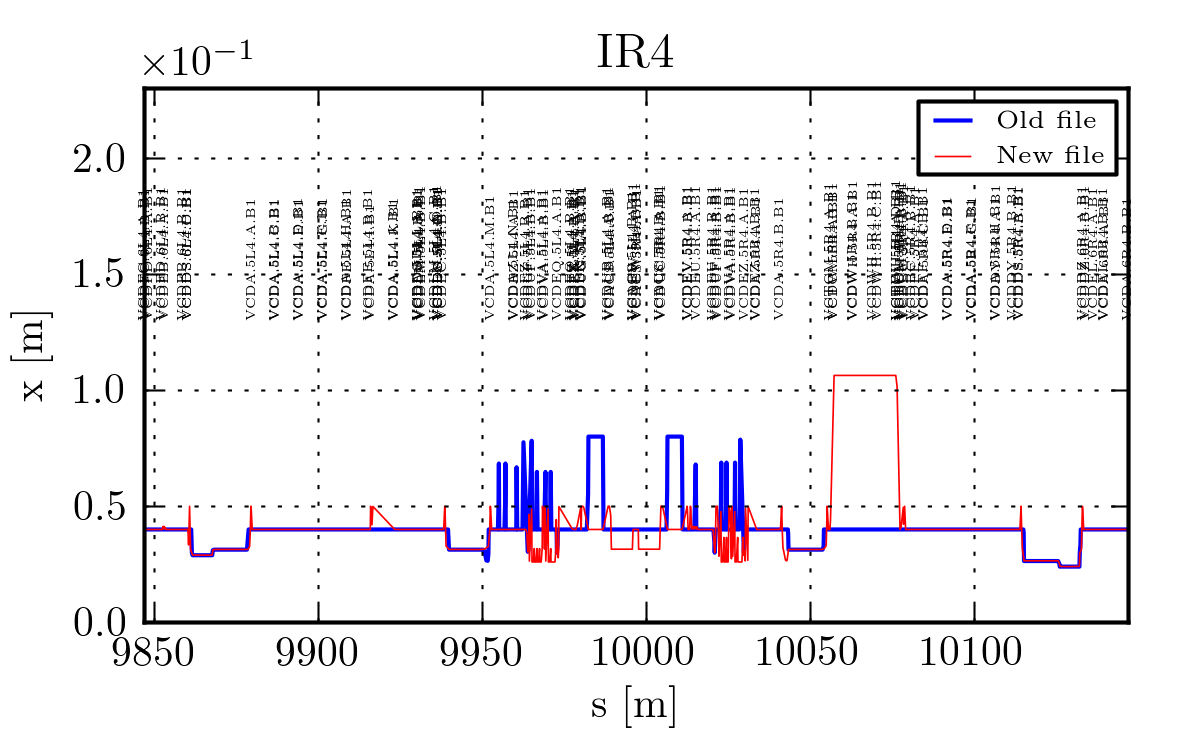
\includegraphics[width=\linewidth]{allapert_ip_4_x_new.png}
\end{minipage}
\begin{minipage}{0.47\linewidth}
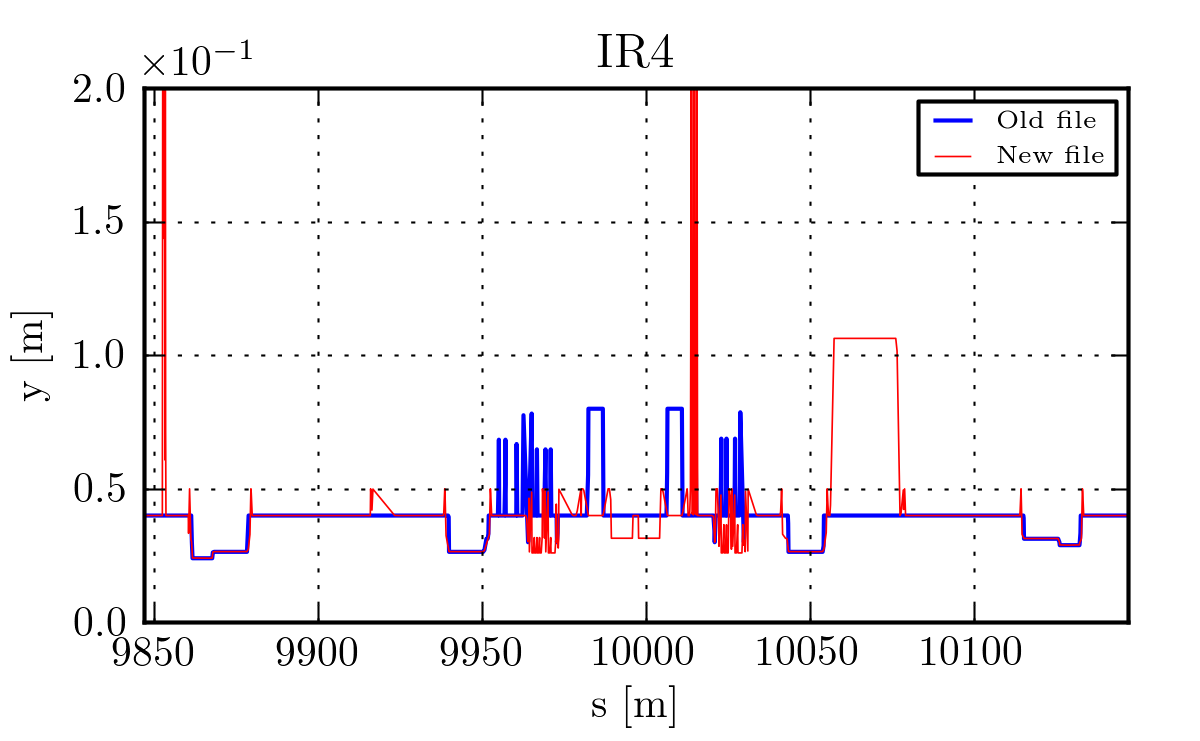
\includegraphics[width=\linewidth]{allapert_ip_4_y_new.png}
\end{minipage}

\begin{minipage}{0.47\linewidth}
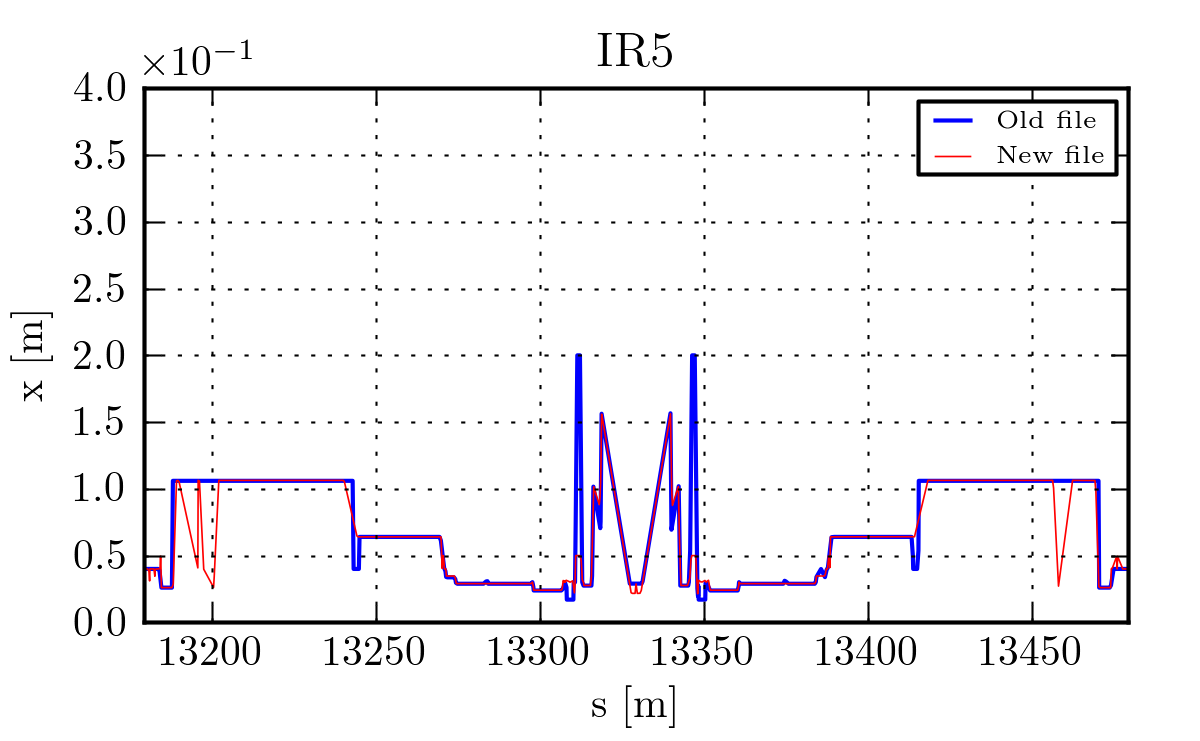
\includegraphics[width=\linewidth]{allapert_ip_5_x_new.png}
\end{minipage}
\begin{minipage}{0.47\linewidth}
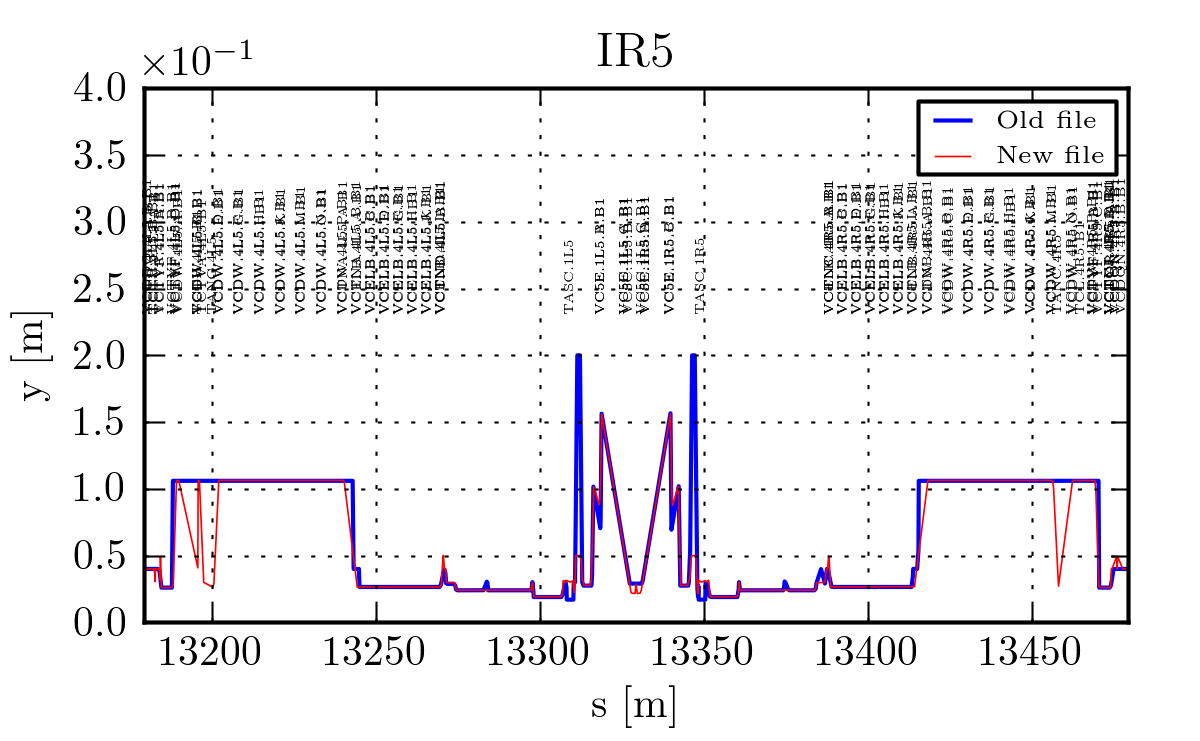
\includegraphics[width=\linewidth]{allapert_ip_5_y_new.png}
\end{minipage}

\begin{minipage}{0.47\linewidth}
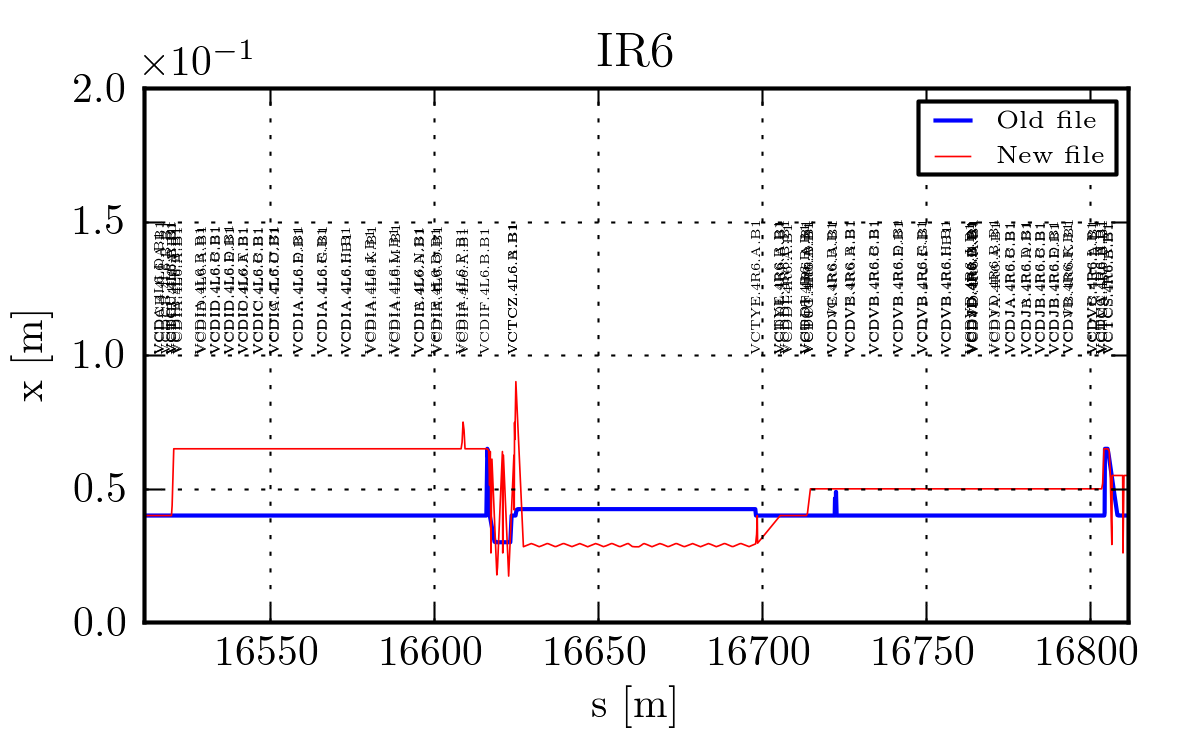
\includegraphics[width=\linewidth]{allapert_ip_6_x_new.png}
\end{minipage}
\begin{minipage}{0.47\linewidth}
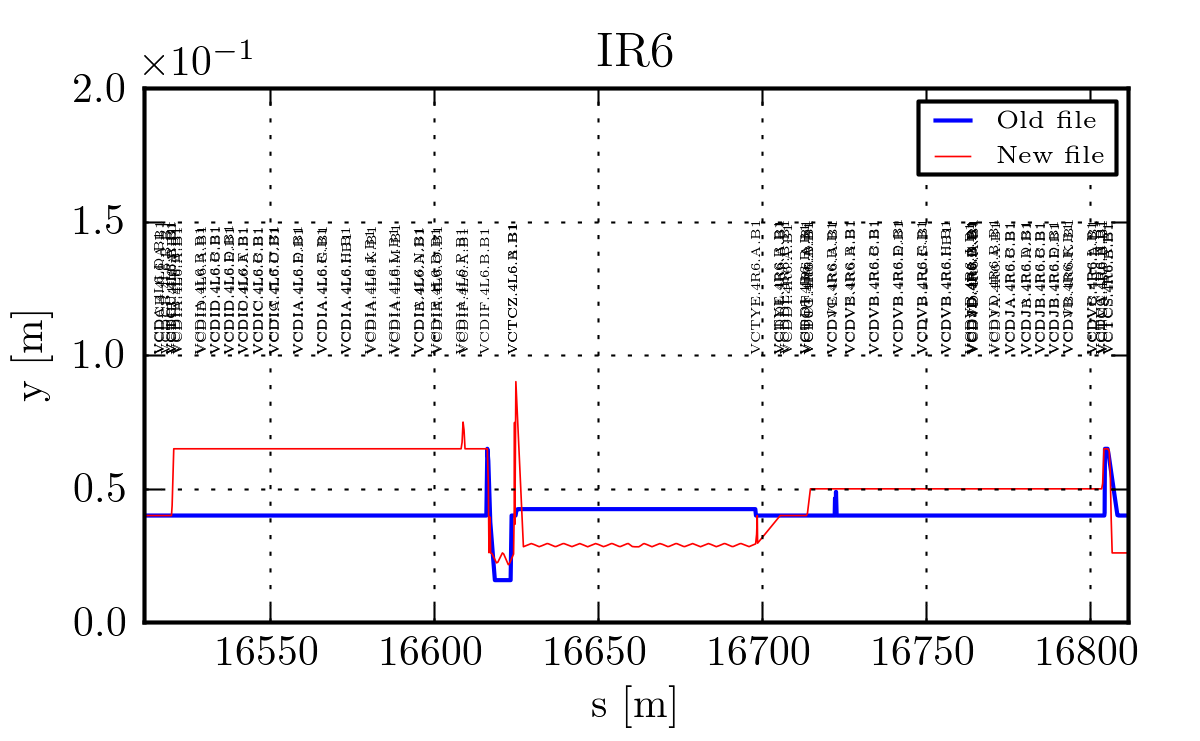
\includegraphics[width=\linewidth]{allapert_ip_6_y_new.png}
\end{minipage}

\begin{minipage}{0.47\linewidth}
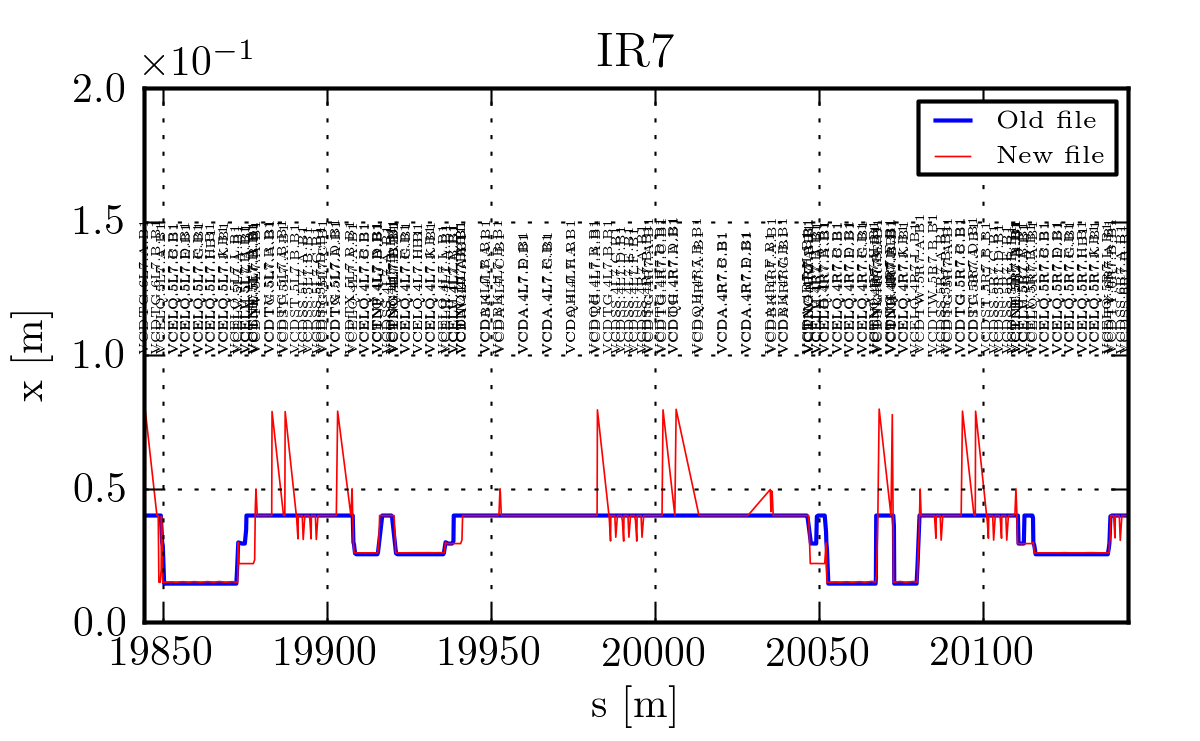
\includegraphics[width=\linewidth]{allapert_ip_7_x_new.png}
\end{minipage}
\begin{minipage}{0.47\linewidth}
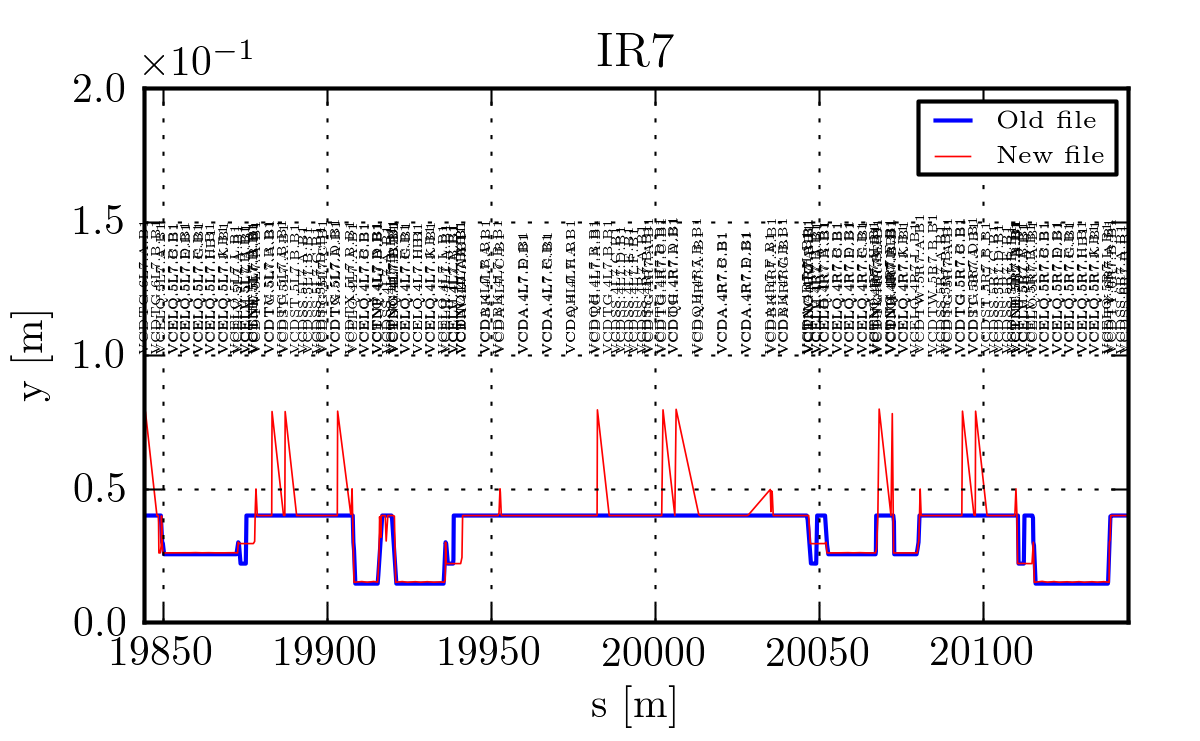
\includegraphics[width=\linewidth]{allapert_ip_7_y_new.png}
\end{minipage}

\begin{minipage}{0.47\linewidth}
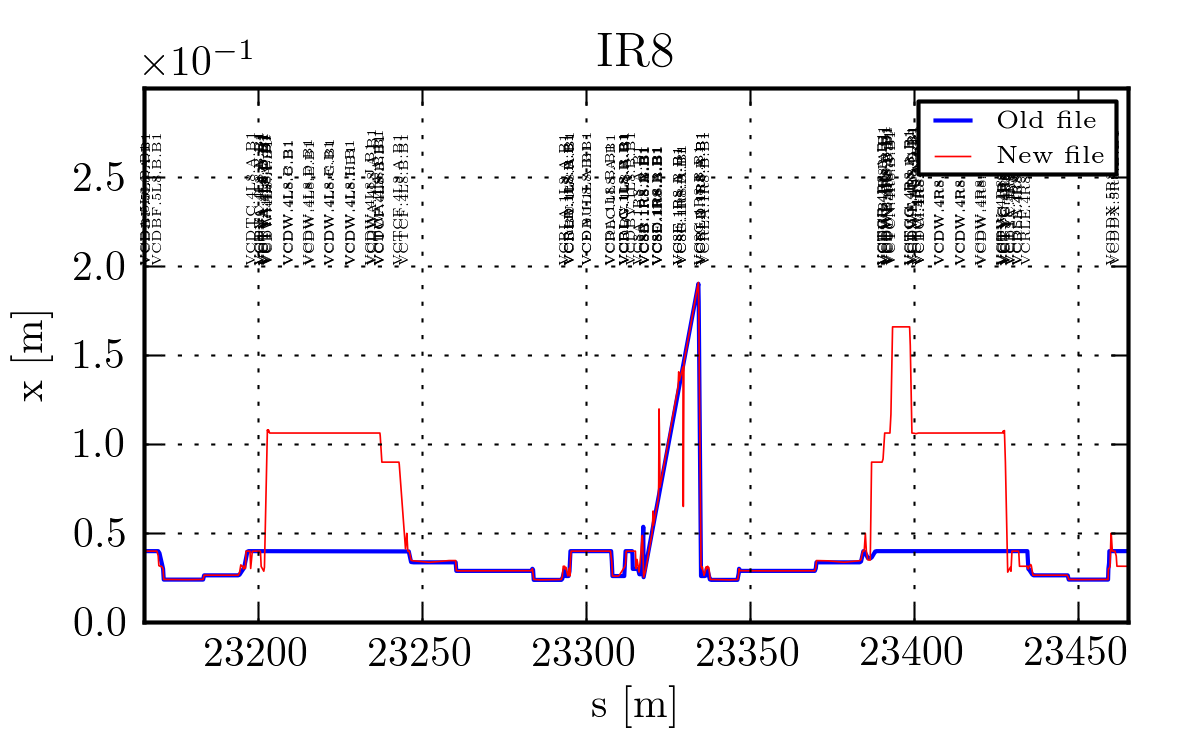
\includegraphics[width=\linewidth]{allapert_ip_8_x_new.png}
\end{minipage}
\begin{minipage}{0.47\linewidth}
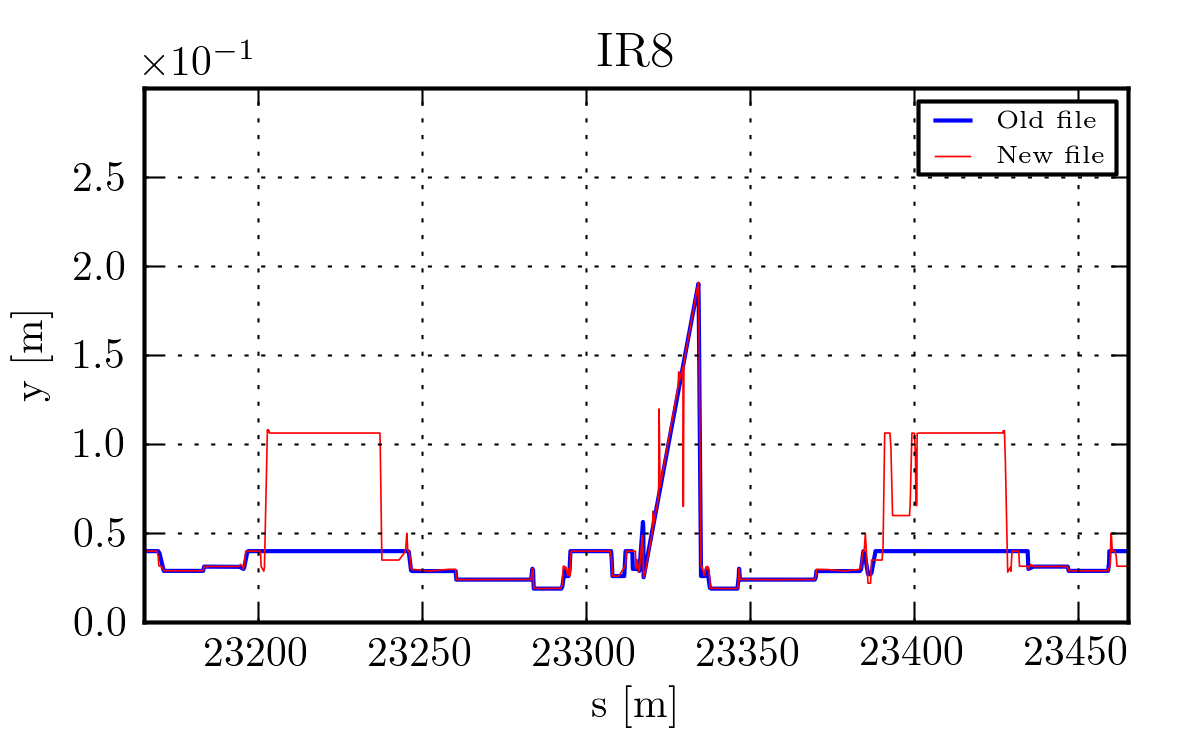
\includegraphics[width=\linewidth]{allapert_ip_8_y_new.png}
\end{minipage}


\subsection{With vacuum markers, experimental beampipe and survey}

\subsection{Without vacuum markers or experimental beampipe}

\bibliography{mybib}
\bibliographystyle{unsrt} 
\end{document}